% =====================================================================
%  J. Giorno -- Economics Letters submission
%  "Wealth effects, perceived stress and crashes without news"
%  ONE self-contained file: figure drawn with pgfplots inside this file,
%  references written out at the end. Single column, numbered sections.
%  Compile: pdflatex Giorno_EL_Crashes_Without_News.tex (run twice)
% =====================================================================
\documentclass[11pt,a4paper]{article}
\usepackage[margin=2.5cm]{geometry}
\usepackage[T1]{fontenc}
\usepackage[utf8]{inputenc}
\usepackage{lmodern}
\usepackage{amsmath,amssymb,amsthm}
\usepackage{booktabs}
\usepackage{threeparttable}
\usepackage{pgfplots}
\pgfplotsset{compat=1.17}
\usepackage{setspace}
\onehalfspacing
\usepackage[authoryear,round]{natbib}
\usepackage[colorlinks=true,linkcolor=black,citecolor=black,urlcolor=black]{hyperref}

\newtheorem{proposition}{Proposition}
\newtheorem{corollary}{Corollary}

\title{\textbf{Wealth effects, perceived stress and crashes without news}}
\author{J.~Giorno\thanks{Graduate Program in Economics, Maring\'a State University (UEM),
Maring\'a, PR, Brazil; and PhDRisk Ltda, Maring\'a, Brazil. E-mail: \texttt{jgiorno@uem.br}.}}
\date{}

\begin{document}
\maketitle

\begin{abstract}
\noindent Many large market falls lack clear news. We show that when levered investors
have wealth effects, the equilibrium price can fold. A closed-form threshold governs when a
fold exists; leverage lowers it, and higher perceived stress shrinks the shock needed to
trigger a crash. Using newspaper codings of 501 S\&P~500 crash days from 1928 to 2022, the
share of crashes without a clear cause rises from 26\% at low predicted stress to 61\% at high
stress ($z=5.6$), robust to crash size and era, though weaker once crisis continuation is
controlled for.
\end{abstract}

\noindent\textbf{Keywords:} crashes; wealth effects; HARA utility; regime switching; news\\
\textbf{JEL classification:} G01, G12, G14, D81

% =====================================================================
\section{Introduction}

Large daily stock market falls often arrive without news that seems large enough to explain
them \citep{CutlerPoterbaSummers1989}. \citet{BBDS2021} coded next-day newspaper accounts of
thousands of large daily moves and found that many have no clear cause. This letter offers a
simple account of \emph{when} such crashes should be common, and tests it.

The mechanism combines two ingredients. Investors who hold the risky asset on leverage have
wealth effects: their risk tolerance falls with their wealth. And all investors share a
filtered belief that the economy is in a stressed regime, which lowers the expected payoff.
We show that wealth effects make excess demand a concave quadratic in price, so the
equilibrium can fold; constant absolute risk aversion rules this out. Higher perceived
stress moves the market towards the fold, so a smaller or less clear shock suffices to
trigger a discontinuous fall. The prediction is that, conditional on a crash, the
probability that it lacks a clear news cause rises with perceived stress.

Our contribution relative to models of wealth effects and amplification
\citep{GennotteLeland1990,KyleXiong2001,BrunnermeierPedersen2009} is a closed-form fold
condition, a sign result for the effect of risk aversion that depends on a wealth pivot, and
a direct link to the observable clarity of crash news. We parameterise preferences in the
Tsallis $q$-exponential form \citep{Tsallis1988}, a HARA utility \citep{Merton1971} in which
one parameter indexes the strength of wealth effects.

% =====================================================================
\section{Model}

A risky asset in supply $S$ has expected payoff $m(\pi)=m_0-\delta\pi$, $\delta>0$, and
payoff variance $v$, where $\pi$ is the commonly filtered probability of the stressed regime
\citep{Hamilton1989}. Levered investors hold $x_0$ shares and cash $c$ ($c<0$ is leverage),
so their wealth at price $P$ is $W(P)=c+x_0P$. Their utility and risk tolerance are
\begin{equation}
u_q(W)=-\big[1-(1-q)\gamma W\big]^{\frac{1}{1-q}},\qquad
T_q(W)=\frac{1}{q\gamma}+\frac{q-1}{q}\,W,
\end{equation}
with $q\ge1$; $q=1$ is CARA and $q>1$ gives decreasing absolute risk aversion. Their demand
is $T_q(W(P))(m(\pi)-P)/v$. Arbitrageurs have limited capacity and demand $A(m_A-P)$, $A>0$.
Market clearing requires
\begin{equation}
Z(P)\equiv T_q\big(W(P)\big)\frac{m(\pi)-P}{v}+A(m_A-P)-S=0 .
\end{equation}

\begin{proposition}\label{prop:cara}
If $q=1$, the equilibrium price is unique and continuous in $\pi$ and in fundamental shocks.
\end{proposition}

\noindent \emph{Proof.} $T_1=1/\gamma$, so $Z'(P)=-1/(\gamma v)-A<0$. \qed

With $\alpha=\frac{1}{q\gamma}+\frac{q-1}{q}c$ and $\beta=\frac{q-1}{q}x_0$, risk tolerance
is $\alpha+\beta P$, and $vZ=0$ becomes the quadratic
$-\beta P^2+(\beta m-\alpha-Av)P+\alpha m+v(Am_A-S)=0$, concave in $P$ for $q>1$. Its
higher root is the stable equilibrium; it disappears when the discriminant vanishes.

\begin{proposition}\label{prop:fold}
A fold exists if and only if
\[
q>q^*\equiv1+\frac{A/\gamma}{x_0(S-Am_A)-Ac}\qquad\big(x_0(S-Am_A)-Ac>0\big),
\]
and the high-price equilibrium exists only for expected payoffs above
\[
m^*=\frac{Av-\alpha+2\sqrt{v\big(\beta(S-Am_A)-\alpha A\big)}}{\beta}.
\]
\end{proposition}

\noindent \emph{Proof.} The discriminant in $P$ is a quadratic in $m$ whose roots are
$[Av-\alpha\pm2\sqrt{v(\beta(S-Am_A)-\alpha A)}]/\beta$; they are real iff
$\beta(S-Am_A)>\alpha A$, which rearranges to $q>q^*$. \qed

\begin{corollary}\label{cor:lev}
$\partial q^*/\partial c>0$: more leverage lowers the threshold for a fold.
\end{corollary}

\begin{proposition}\label{prop:sign}
At a fold with price $P^*$ and wealth $W^*=c+x_0P^*$, $\operatorname{sign}(dm^*/dq)=
\operatorname{sign}(1/\gamma-W^*)$.
\end{proposition}

\noindent \emph{Proof.} At the fold $Z=Z_P=0$, so $dm^*/dq=-Z_q/Z_m$, with $Z_m=T_q/v>0$
and $Z_q=(W^*-1/\gamma)(m^*-P^*)/(q^2v)$ since $\partial T_q/\partial q=(W-1/\gamma)/q^2$;
investors are long, so $m^*>P^*$. \qed

\medskip
Proposition~\ref{prop:sign} reflects a wealth pivot: a rise in $q$ raises absolute risk
aversion for investors with $W<1/\gamma$ and lowers it above. Greater risk aversion
therefore moves the market towards the fold only when levered wealth is low.

Let fundamental shocks $\varepsilon$ with density $f$ and survival function $\bar F$ arrive
at rate $\lambda_s$. For $q>q^*$, a crash occurs when $\varepsilon>m_0-\delta\pi-m^*$, so
crash intensity is $\lambda(\pi)=\lambda_s\bar F(m_0-\delta\pi-m^*)$. \emph{The shock needed to
trigger a crash falls one-for-one with $\delta\pi$.} News that is large and clear crosses
the threshold whatever the state; news that is small or unclear crosses it only when $\pi$
is high. Hence:

\medskip
\noindent\textbf{Prediction.} \emph{Conditional on a crash, the probability that it lacks a
clear news cause increases with perceived stress.}

\medskip
\noindent In a calibration ($\gamma=2$, $v=1$, $c=-0.3$, $x_0=1$, $A=0.15$, $m_A=0.6$,
$S=1$), $q^*=1.079$; with $q=1$ the price falls smoothly as $m$ declines, while with $q=1.5$
it drops by 0.91 at $m^*=2.858$. Across 17{,}093 random parameter draws with a relevant fold,
the sign in Proposition~\ref{prop:sign} held in every case.

% =====================================================================
\section{Evidence}

\subsection{Data}

We use daily S\&P~500 closes from 1928 to 2022 and the newspaper codings of \citet{BBDS2021},
which record, for every US daily move larger than 2.5\% in absolute value, a continuous index
of how clearly journalists identified its cause. We match 501 downward jumps and call a crash
\emph{low-clarity} if its index is below the sample median. Perceived stress is the predicted
probability $b^-_t$ of the high-volatility state from a two-state Gaussian hidden Markov model
of daily returns \citep{Hamilton1989}, computed with the forward filter, so it uses only
information up to $t-1$. Standard errors are from case bootstraps.

\subsection{Results}

Figure~\ref{fig:clarity} shows the main pattern. The share of low-clarity crashes rises from
26\% when $b^-_t\le0.2$ to 61\% when $b^-_t>0.8$. A probit of the low-clarity indicator on
$b^-_t$ across crash days gives a coefficient of 0.99 ($z=5.6$).

\begin{figure}[ht]
\centering
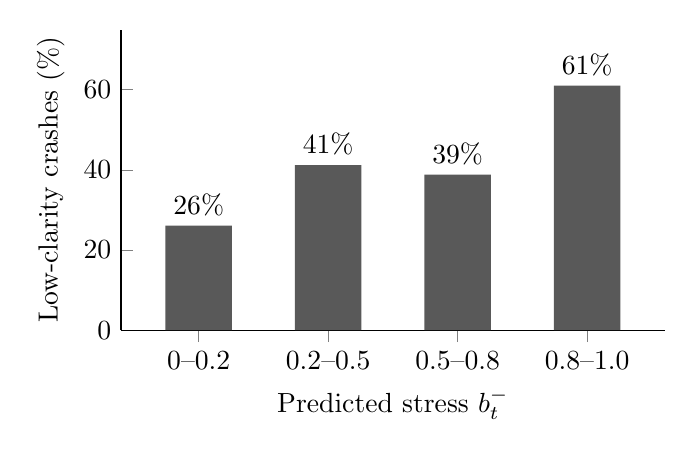
\begin{tikzpicture}
\begin{axis}[
  ybar, bar width=24pt, width=0.7\textwidth, height=5.4cm,
  ymin=0, ymax=75, ylabel={Low-clarity crashes (\%)},
  xlabel={Predicted stress $b^-_t$},
  symbolic x coords={0--0.2,0.2--0.5,0.5--0.8,0.8--1.0}, xtick=data,
  nodes near coords={\pgfmathprintnumber[fixed,precision=0]{\pgfplotspointmeta}\%},
  axis lines*=left, enlarge x limits=0.2]
\addplot[fill=black!65,draw=none] coordinates {(0--0.2,26.1) (0.2--0.5,41.2) (0.5--0.8,38.8) (0.8--1.0,61.0)};
\end{axis}
\end{tikzpicture}
\caption{Share of S\&P~500 downward jumps (below $-2.5\%$) without a clear news cause, by
predicted stress on the crash day, 1928--2022. Crash days per bin: 88, 51, 67, 295.}
\label{fig:clarity}
\end{figure}

\begin{table}[ht]
\centering
\begin{threeparttable}
\caption{Probit of low clarity on predicted stress, crash days 1928--2022}
\label{tab:robust}
\small
\begin{tabular}{lcc}
\toprule
Controls & Coefficient on $b^-_t$ & $z$ \\
\midrule
None & 0.987 & 5.56 \\
Crash size relative to recent volatility & 0.947 & 4.56 \\
+ era dummies (1946--96, 1997--2022) & 0.820 & 3.70 \\
+ linear time trend & 0.814 & 3.68 \\
+ crash in previous five days & 0.441 & 1.68 \\
First crashes only ($n=276$), size and era & 0.493 & 1.62 \\
\bottomrule
\end{tabular}
\begin{tablenotes}\footnotesize
\item $n=501$ crash days unless stated. Size is $|r_t|/\hat\sigma_{t-1}$ with EWMA volatility
($\lambda=0.94$). Case-bootstrap standard errors.
\end{tablenotes}
\end{threeparttable}
\end{table}

Table~\ref{tab:robust} reports robustness. The effect survives controls for the size of the
crash relative to recent volatility, so it does not merely reflect large moves being more
newsworthy; it survives era dummies and a time trend, so it is not driven by the secular rise
in news clarity documented by \citet{BBDS2021}. It holds within each era: the low-clarity
share rises from 47\% to 75\% (1928--45), from 30\% to 49\% (1946--96) and from 20\% to 27\%
(1997--2022) between low ($b^-_t\le0.5$) and high stress.

Controlling for a crash in the previous five days halves the coefficient ($z=1.7$); among
first crashes only, the low-clarity share is 30.3\% at low stress and 45.8\% at high stress
($z=1.6$). Part of the effect therefore comes from crashes that follow other crashes without
new news. This is consistent with the self-reinforcing dynamics the model implies, but also
with journalists having nothing new to report during a sell-off, and our data cannot separate
the two.

Two further implications are not supported in preliminary tests. Using FINRA margin debt
(1997--2026) as a leverage proxy, the sensitivity of crash probability to perceived stress
does not rise with leverage; and crash probability is not convex in $b^-_t$. Retail margin
debt may measure the wrong leverage: the investors near a fold are mostly levered
institutions \citep{AdrianEtulaMuir2014}.

% =====================================================================
\section{Conclusion}

Wealth effects make equilibrium prices capable of folding, and perceived stress brings the
market closer to the fold, so smaller and less clear news suffices to cause a crash. A century
of US crash news supports this prediction, although part of the effect reflects crisis
continuation. The model's leverage predictions call for tests with institutional leverage
data.

% =====================================================================
\section*{Declaration of competing interest}
The author declares no competing financial interests or personal relationships that could
have appeared to influence the work reported in this paper.

\section*{Data availability}
Data are from Yahoo Finance (S\&P~500), FINRA (margin statistics) and \citet{BBDS2021}.
Code reproducing all results is available at [repository URL to be added].

\section*{Declaration of generative AI and AI-assisted technologies in the writing process}
During the preparation of this work the author used [name of tool] in order to [reason].
After using this tool, the author reviewed and edited the content as needed and takes full
responsibility for the content of the publication.

% =====================================================================
\begin{thebibliography}{99}
\small

\bibitem[Adrian et~al.(2014)]{AdrianEtulaMuir2014}
Adrian, T., Etula, E., Muir, T., 2014. Financial intermediaries and the cross-section of
asset returns. Journal of Finance 69, 2557--2596.

\bibitem[Baker et~al.(2021)]{BBDS2021}
Baker, S.R., Bloom, N., Davis, S.J., Sammon, M.C., 2021. What triggers stock market jumps?
NBER Working Paper 28687.

\bibitem[Brunnermeier and Pedersen(2009)]{BrunnermeierPedersen2009}
Brunnermeier, M.K., Pedersen, L.H., 2009. Market liquidity and funding liquidity. Review of
Financial Studies 22, 2201--2238.

\bibitem[Cutler et~al.(1989)]{CutlerPoterbaSummers1989}
Cutler, D.M., Poterba, J.M., Summers, L.H., 1989. What moves stock prices? Journal of
Portfolio Management 15, 4--12.

\bibitem[Gennotte and Leland(1990)]{GennotteLeland1990}
Gennotte, G., Leland, H., 1990. Market liquidity, hedging, and crashes. American Economic
Review 80, 999--1021.

\bibitem[Hamilton(1989)]{Hamilton1989}
Hamilton, J.D., 1989. A new approach to the economic analysis of nonstationary time series
and the business cycle. Econometrica 57, 357--384.

\bibitem[Kyle and Xiong(2001)]{KyleXiong2001}
Kyle, A.S., Xiong, W., 2001. Contagion as a wealth effect. Journal of Finance 56,
1401--1440.

\bibitem[Merton(1971)]{Merton1971}
Merton, R.C., 1971. Optimum consumption and portfolio rules in a continuous-time model.
Journal of Economic Theory 3, 373--413.

\bibitem[Tsallis(1988)]{Tsallis1988}
Tsallis, C., 1988. Possible generalization of Boltzmann--Gibbs statistics. Journal of
Statistical Physics 52, 479--487.

\end{thebibliography}

\end{document}
